\documentclass[onecolumn,10pt,cleanfoot]{asme2ej}

\usepackage{graphicx} %% for loading jpg figures
\usepackage{bm}
\usepackage{nicefrac}
\usepackage{mathtools}
\usepackage{amssymb}
\usepackage{amsmath}
\usepackage{parskip}
\usepackage{listings}
\usepackage{tablefootnote}
\usepackage{float}
\usepackage{xcolor}
\usepackage{xurl}

\title{Bias variance trade-off comparison of regression models}

%%% first author
\author{Jonatan H. Hanssen
    \affiliation{
	Bachelor Student, Robotics and \\
	Intelligent Systems\\ \\[-10pt]
	Department of Informatics\\ \\[-10pt]
	The faculty of Mathematics and \\
	Natural Sciences\\ \\[-10pt]
    Email: jonatahh@ifi.uio.no
    }
}

\author{Eric E. Reber
    \affiliation{
	Bachelor Student, Robotics and \\
	Intelligent Systems\\ \\[-10pt]
	Department of Informatics\\ \\[-10pt]
	The faculty of Mathematics and \\
	Natural Sciences\\ \\[-10pt]
    Email: ericer@ifi.uio.no
    }
}

\author{Gregor Kajda
    \affiliation{
	Bachelor Student, Robotics and \\
	Intelligent Systems\\ \\[-10pt]
	Department of Informatics\\ \\[-10pt]
	The faculty of Mathematics and \\
	Natural Sciences\\ \\[-10pt]
    Email: grzegork@ifi.uio.no
    }
}


\begin{document}


\maketitle


\section{Abstract}
Comparing the different regression methods of OLS and ridge regression, we found the regularization provided by ridge regression to decrease our MSE by 14\% by studying the bias variance trade-off of these methods. Regularization was sufficient for delaying overfitting, but a too large regularization value could increase the MSE unnecessarily. Furthermore, decision trees yielded poor results for our regression problem, more than doubling the MSE of our results found by ridge regression. We turned to neural networks, which were also unable to beat the results obtained with ridge regression even when using a very complex architecture consisting of 5 hidden layers. Ridge regression took the crown with an MSE of 0.0031.

\section{Introduction}
In regression, we wish to create a general model that provides a low MSE even for data that it was not trained on. To study this attribute, we observe the bias variance trade-off of a given regression model to understand where our model begins to overfit to the training data. Understanding the bias variance trade-off allows us to study the relationship between model complexity and the test MSE score of our model, aiding in model selection. In this paper, we will compare the bias variance trade-offs of ordinary least squares and ridge regression methods, along with neural networks and decision trees applied for regression. We want to see how far we can push the complexities of our models without overfitting, along with understanding which model can provide the lowest MSE of the test data.

First, we will explain the theory and method used in this paper, followed up by a critical discussion of our results. Finally, we will write a conclusion summarizing our core results and lessons.

\section{Method}

\subsection{Theory}

This sections covers the theoretic background which underlies the methods used in this paper.

\subsubsection{Linear Regression}

Linear regression aims to find a relationship between a set of dependent and explanatory variables. Assume we have a dataset, which contains a series of inputs $\{x_i\}$, and corresponding target values $\{y_i\}$. Our assumption is that there is some relationship $y_i = f(x_i) + \epsilon_i$ where $\epsilon_i \sim N(0,\sigma^2)$, and we wish to create a model which approximates this relationship. More specifically, we wish to find a vector $\beta$ which gives us the "best" approximation $\bm{\tilde{y}}$ of $\bm{y}$, by using the parameters in the following equation:

\begin{equation}
X \bm{\beta} = \bm{\tilde{y}}
\label{first}
\end{equation}

Here, $X$ is our design matrix, containing our explanatory variables, our features, while $\bm{\tilde{y}}$ is our predicted vector. By defining a cost function, such as Mean Squared Error, we are able to find the parameter $\beta$ which minimizes the difference between our prediction and the target values. By using the normal equations, we can solve this problem analytically.

\subsubsection{Ridge Regression}

A common problem with OLS is what is known as overfitting (we will discuss this in greater detail in later sections). A symptom of overfitting is that the values in the parameter vector $\bm{\beta}$ grow very large, and vary wildly for small changes in our dataset. To counteract this, we can add to the cost function a term which increases with the values in $\bm{\beta}$. Optimizing the cost function would now not only mean finding the smallest difference between target and predicted values, but also minimizing the absolute value of the parameters. We now define a new cost function

\begin{equation}
	C_{lasso}(\bm{\beta}) = \sum_{i=0}^{n-1}(y_i-X_{i*}\bm{\beta})^2 + \lambda \sum_{j=0}^{p-1} \beta_j^2
\end{equation}

$||\beta||_2^2$ is equal to $\beta^T\beta$ and is simply the norm of the parameter vector, squared. With the new hyperparameter $\lambda \in (0, \inf)$ , we can decide how harshly we should punish large values in our parameter vector. Finding an optimal $\lambda$ is an important step in the process of finding the best parameters for our model.

\subsubsection{Feedforward Neural Networks}

For some problems, it is sufficient to choose a set of basis functions and find their optimal linear combination. Given that our problem can be reasonably approximated by this basis, we can achieve good results. However, by limiting ourselves to linear functions, we are possibly limiting our model, as our dataset may well be better approximated by a different basis, or perhaps not even by a linear combination of functions at all. Because of this, linear regression is not able to understand the interaction between two arbitrary input variables \cite[165]{gbc}. A better approach would be to simply feed our model our features directly, and hope that it may somehow learn the relationship organically.

To learn any arbitrary relationship between our features may at first seem like an intractable problem, but we are actually able to achieve this with relatively small changes to our linear regression methods. Instead of having our prediction vector be a linear combination of our input vector, we use the linear combinations of the inputs to create an intermediate vector, and apply an activation function to this vector. The resulting values from this function are either passed to the output as a linear combination again, or sent to another intermediate vector. By having the activation function be a nonlinear function, such as the sigmoid or RELU function, we are able to approximate any continous function to arbitrary accuracy \cite[230]{cmb}. By introducing these intermediate vectors, we have created a layered structure, where information is fed forward from layer to layer. Because of this, we call this model a Multilayer Perceptron or a Feedforward Neural Network.

Mathematically, each node on a layer is a linear combination of all the nodes of the previous layer, fed into the activation function for the current layer.

\subsubsection{Decision trees}
A decision tree will split our dataset, the predictor space, into different non-overlapping areas for which we will make the yield the same prediction for every observation that falls into this area. The prediction will be the average of the observations present in the area during training. The areas, or regions, are chosen to minimize the MSE. The decision tree has an advantage of being very intuitive and explainable, as the observations are placed into these regions using simple conditions.

\subsubsection{Bootstrap}

Bootstrap is a resampling method divided into simple steps. First, we reshuffle our dataset with replacement, which will provide us with a new dataset. Note that we will already have split our data into train and test data before we begin the bootstrap, so when we reshuffle, we will only reshuffle the training data. The reshuffled datasets act as our samples.

Secondly, we will perform our linear regression on this new dataset and store the predictions of the test data. Thirdly, we repeat for a given large number of iterations. Since we use all the test predictions to calculate the MSE, bias and variance, we will then according to the central limit theorem \cite{CLT} obtain a normal distribution of these performance metrics. The law of large numbers \cite{LLN} then tells us that the mean sample values of the MSE, bias and variance approach the true value of MSE, bias and variance. This is dependent on our assumption that our data is independently and identically distributed.

These approximations of the true value of MSE, bias and variance will become useful when performing our bias-variance trade-off analysis.

\subsubsection{Bias-variance trade-off}

A crucial part of model evaluation is ensuring that the model is neither underfitted nor overfitted, which we can determine by observing the relationship between the bias and the variance. Bias is defined as $(Bias[\tilde{y}])^2 = (y-E[\tilde{y}])^2$, the difference between the expected value of our prediction and the observed value. Models with high bias are usually underfitted, whilst models with low bias are the opposite. Variance on the other hand is defined as $var[\tilde{f}] = \frac{1}{n}\sum(\tilde{y_i}-E[\tilde{y}])^2$, how far away predictions are from the mean prediction. Models with high variance are usually overfitted to the training data, whilst low variance models are the opposite.

A good rule of thumb for finding a good fit is looking at the intercept between bias and variance. This is because the cost function can be decomposed into these two elements.

\subsection{Implementation}

Our implementation can be found at \texttt{https://github.com/EricEReber/Bias-variance.git}.

To obtain a valid comparison accross the various regression methods, we used methods found in scikit learn's machine learning library such as  LinearRegression, Ridge, MLPRegressor and DecisionTreeRegressor. We specify the model we wish to use such that it outputs a mean squared error as it increases in complexity. The complexity for OLS and ridge is the polynomial degree up to which we create the design matrix, the model complexity for the feed forward neural network is the amount of hidden nodes in our hidden layers, and the complexity in the decision tree is represented by its depth. For the feed forward neural network we implemented both one and two hidden layers, and distributed the hidden nodes equally across the layers. The feed forward neural network is trained for 2000 epochs using the logistic activation function and the adam scheduler.

Each model is bootstrapped using our own wrapper function for 100 bootstraps.

\subsection{Datasets}

Below is a short description of each dataset used in this report, along with a table (Table.~\ref{datasettable}) listing their characteristics.

\subsubsection{Franke Function}

The Franke Function is a simple weighted sum of exponentials, taking two inputs and returning a real value. It is commonly used to test machine learning algorithms for regression problems. For OLS and ridge regression, our training data will be based on a 9th degree polynomial fit of the Franke Function, with 56 features. For the feed forward neural network and decision tree, we will use the x and y values directly. The Franke Function is defined as follows.


\begin{multline}
f(x,y) = \frac{3}{4}e^{\left(-\frac{(9x-2)^2}{4}-\frac{(9y-2)^2}{4}\right)} +  \frac{3}{4}e^{\left(-\frac{(9x+1)^2}{49}-\frac{(9y+1)}{10}\right)} +
\frac{1}{2}e^{\left(-\frac{(9x-7)^2}{4}-\frac{(9y-3)^2}{4}\right)} - 
\frac{1}{5}e^{\left(-(9x-4)^2-(9y-7)^2\right)}.
\end{multline}

In practice, to better test our models ability to generalize and to mimic real terrain data, we add a normally distributed noise $N(0,0.05)$ to this function.

\section{Results}

\begin{figure}[H]
\centerline{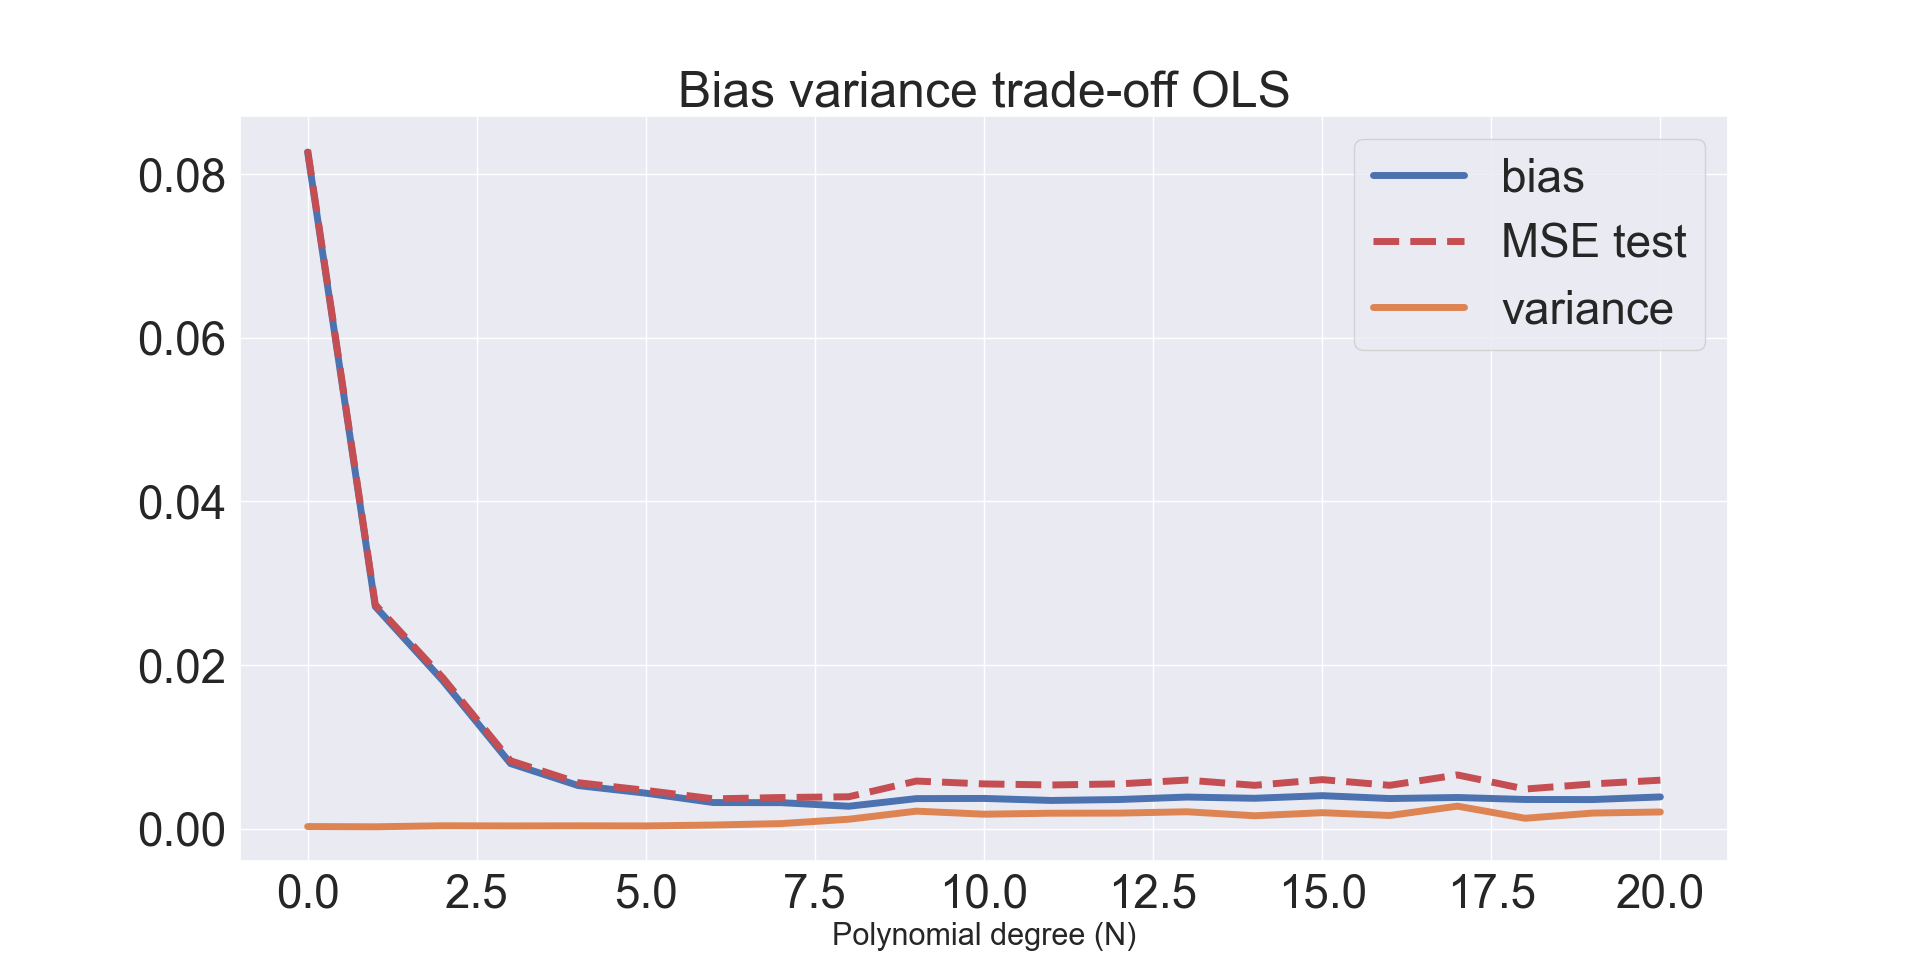
\includegraphics[width=5in]{figs/BV_OLS.png}}
\caption{Bias variance trade-off for ordinary least squares linear regression. Y axis represents model complexity as polynomial degrees.}
\label{OLS}
\end{figure}

We observe for (Fig.~\ref{OLS}) that the variance does not increase greatly over the model complexity, and that bias and variance never cross. However, this is simply a thumb rule and we can observe that the test MSE begins to rise once the bias is low and the variance begins increasing, meaning that we can see slight overfitting occuring around polynomial degree 7. The lowest test MSE, found just before the overfitting occures at polynomial degree 6, is 0.0036. Ordinary least squares does not make an attempt to stop overfitting using regularization, so in order to observe how the bias variance changes when introducing a regularization hyperparameter we turn to ridge regression.

\begin{figure}[H]
\centerline{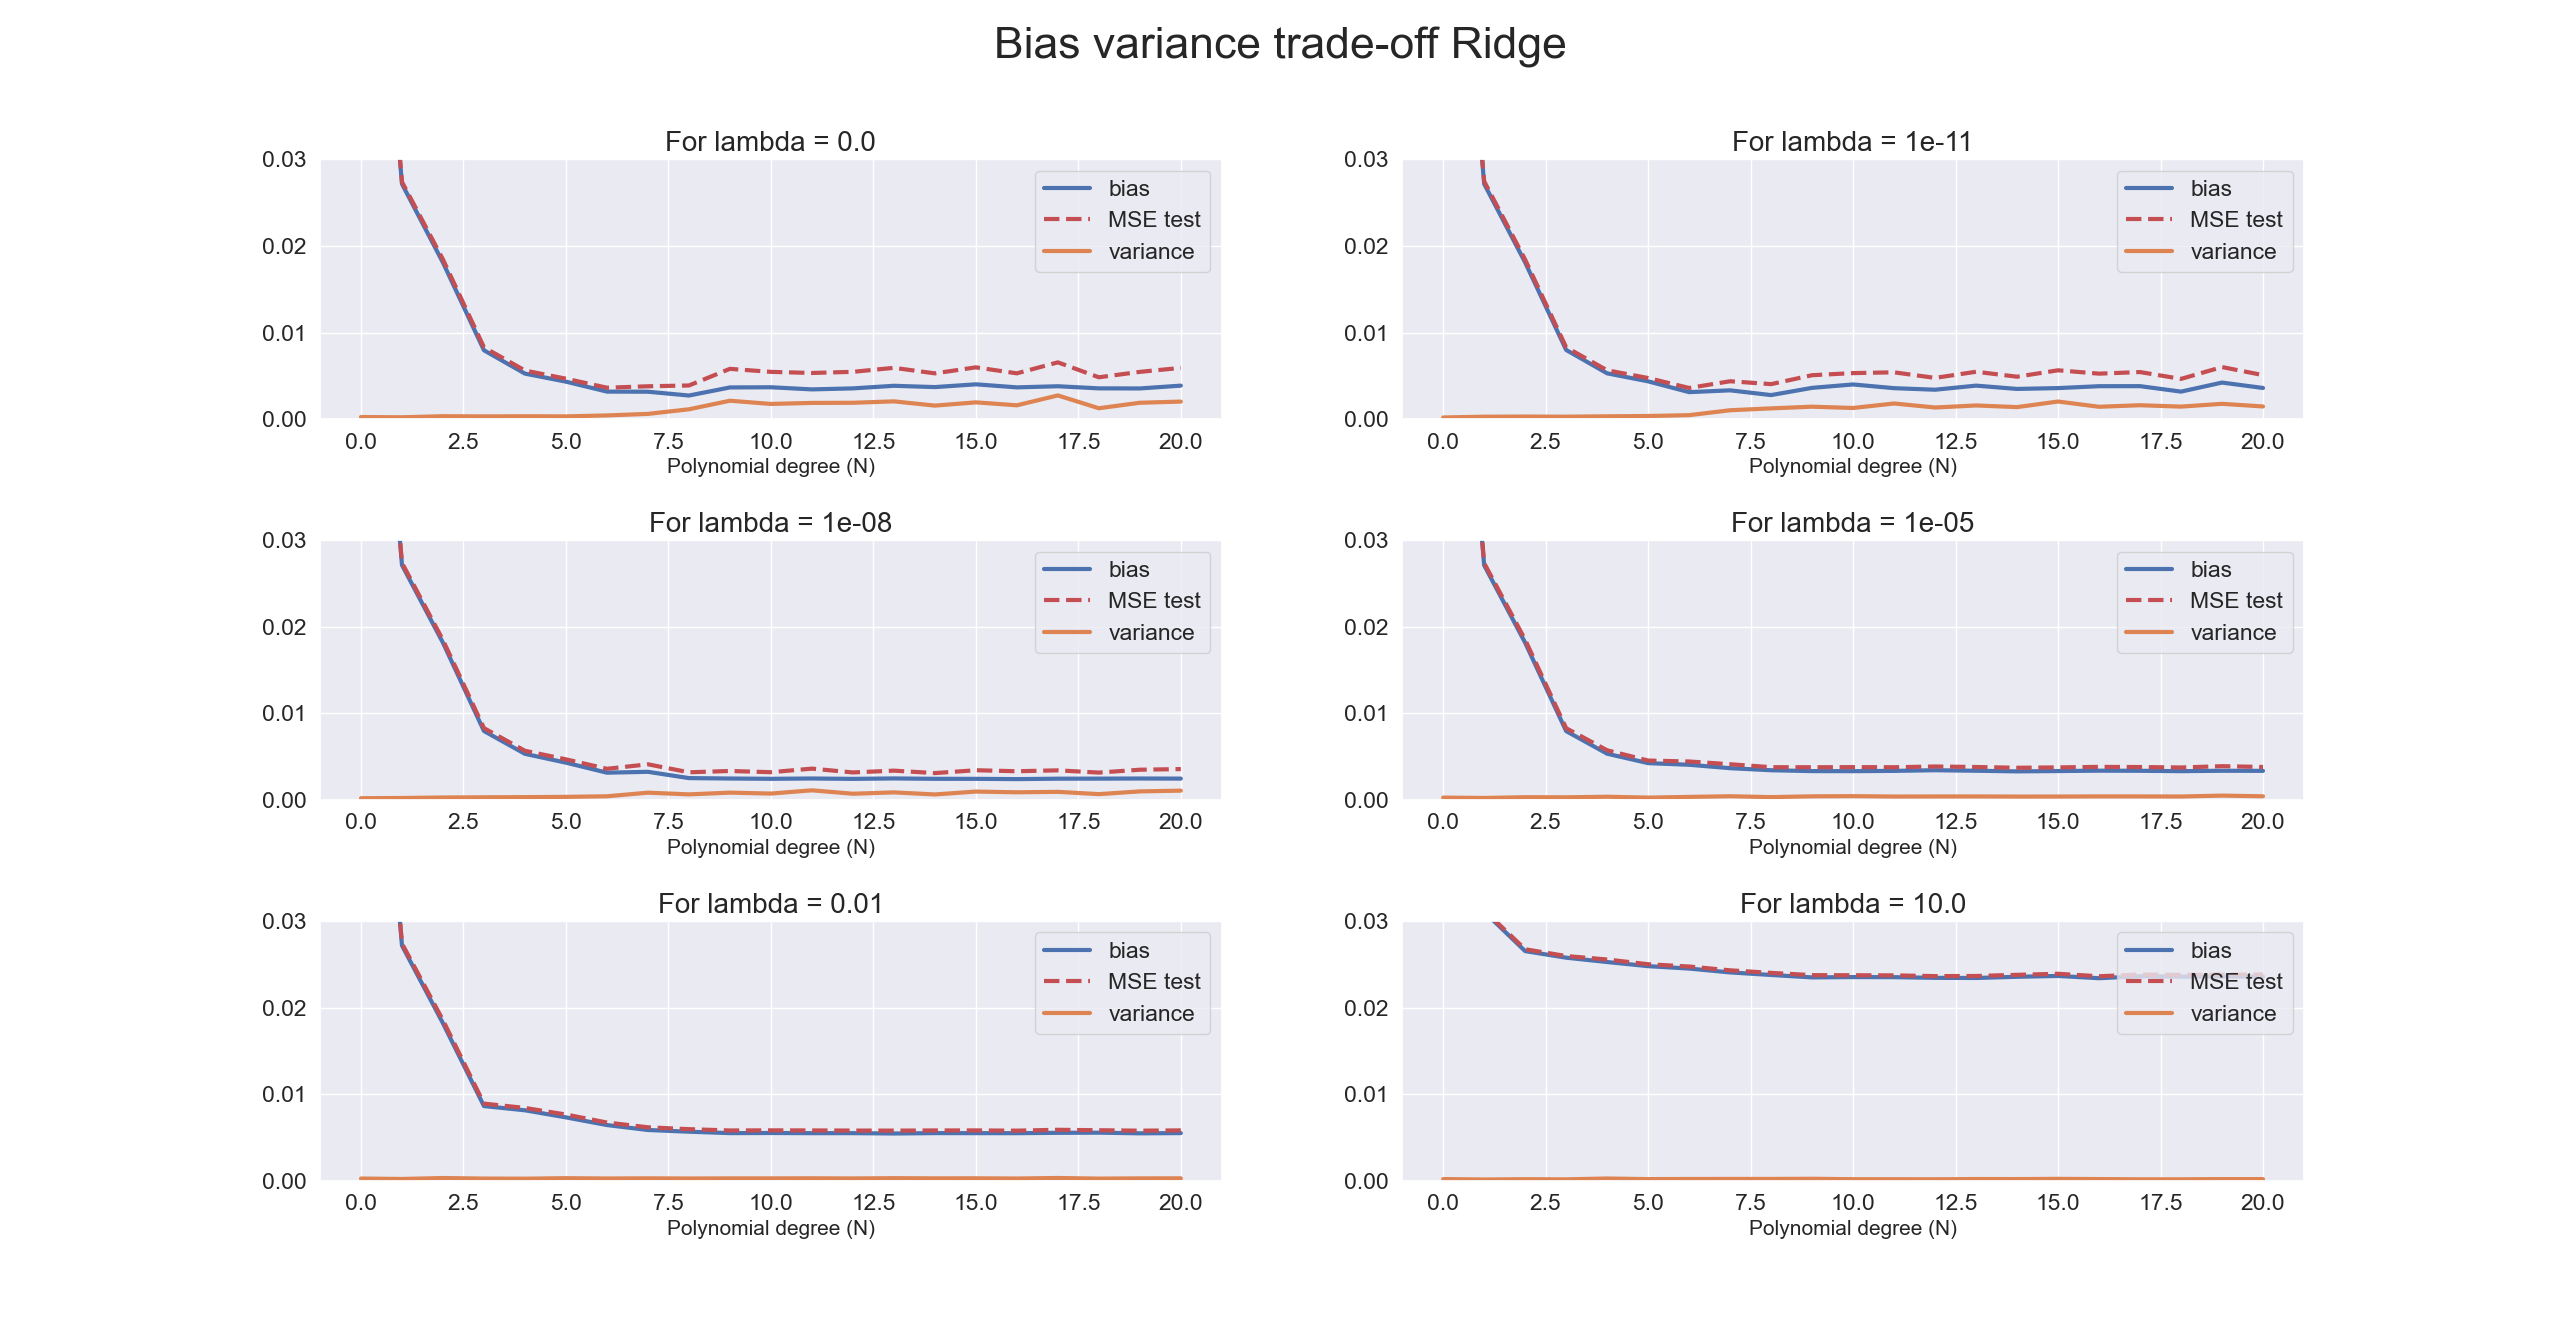
\includegraphics[width=9in]{figs/BV_Ridge.png}}
\caption{Bias variance trade-off for ridge regression. Y axis represents model complexity as polynomial degrees.}
\label{Ridge}
\end{figure}

By introducing different levels of regularization, we can see from (Fig.~\ref{Ridge}) that the regularization hyperparameter delays overfitting for $\lambda \geq 1e-08$, yielding both a low bias and variance. With this improvement, obtain a minimal test MSE for $\lambda = 1e-08$ of 0.0031 at polynomial degree 14. This yields a 14\% decrease in MSE from OLS' MSE of 0.0036, a significant improvement. For $\lambda = 0$ however, we observe the same bias variance trade-off as ordinary least squares, which is expected considering that ridge regression is equivalent with OLS if the regularization term is 0. As we increase the regularization term, overfitting is delayed, but the test MSE stays at higher values as the bias never decreases for the given range of model complexities. For high values of lambda, such as $\lambda \geq 0.01$ as seen in (Fig.~\ref{Ridge}), the test MSE is larger than the overfitted MSE of  OLS. Thus, regularization does not always provide an improvement, but for the correct hyperparameter value it provides a significantly lower MSE. It should also be mentioned that in order to get this 14\% decrease in MSE over OLS, a more complex and thus computationally heavy model is required. However, as ridge has an analytical solution this simply requires a slightly larger matrix inversion, which won't break the bank for the Franke function.

\begin{figure}[H]
\centerline{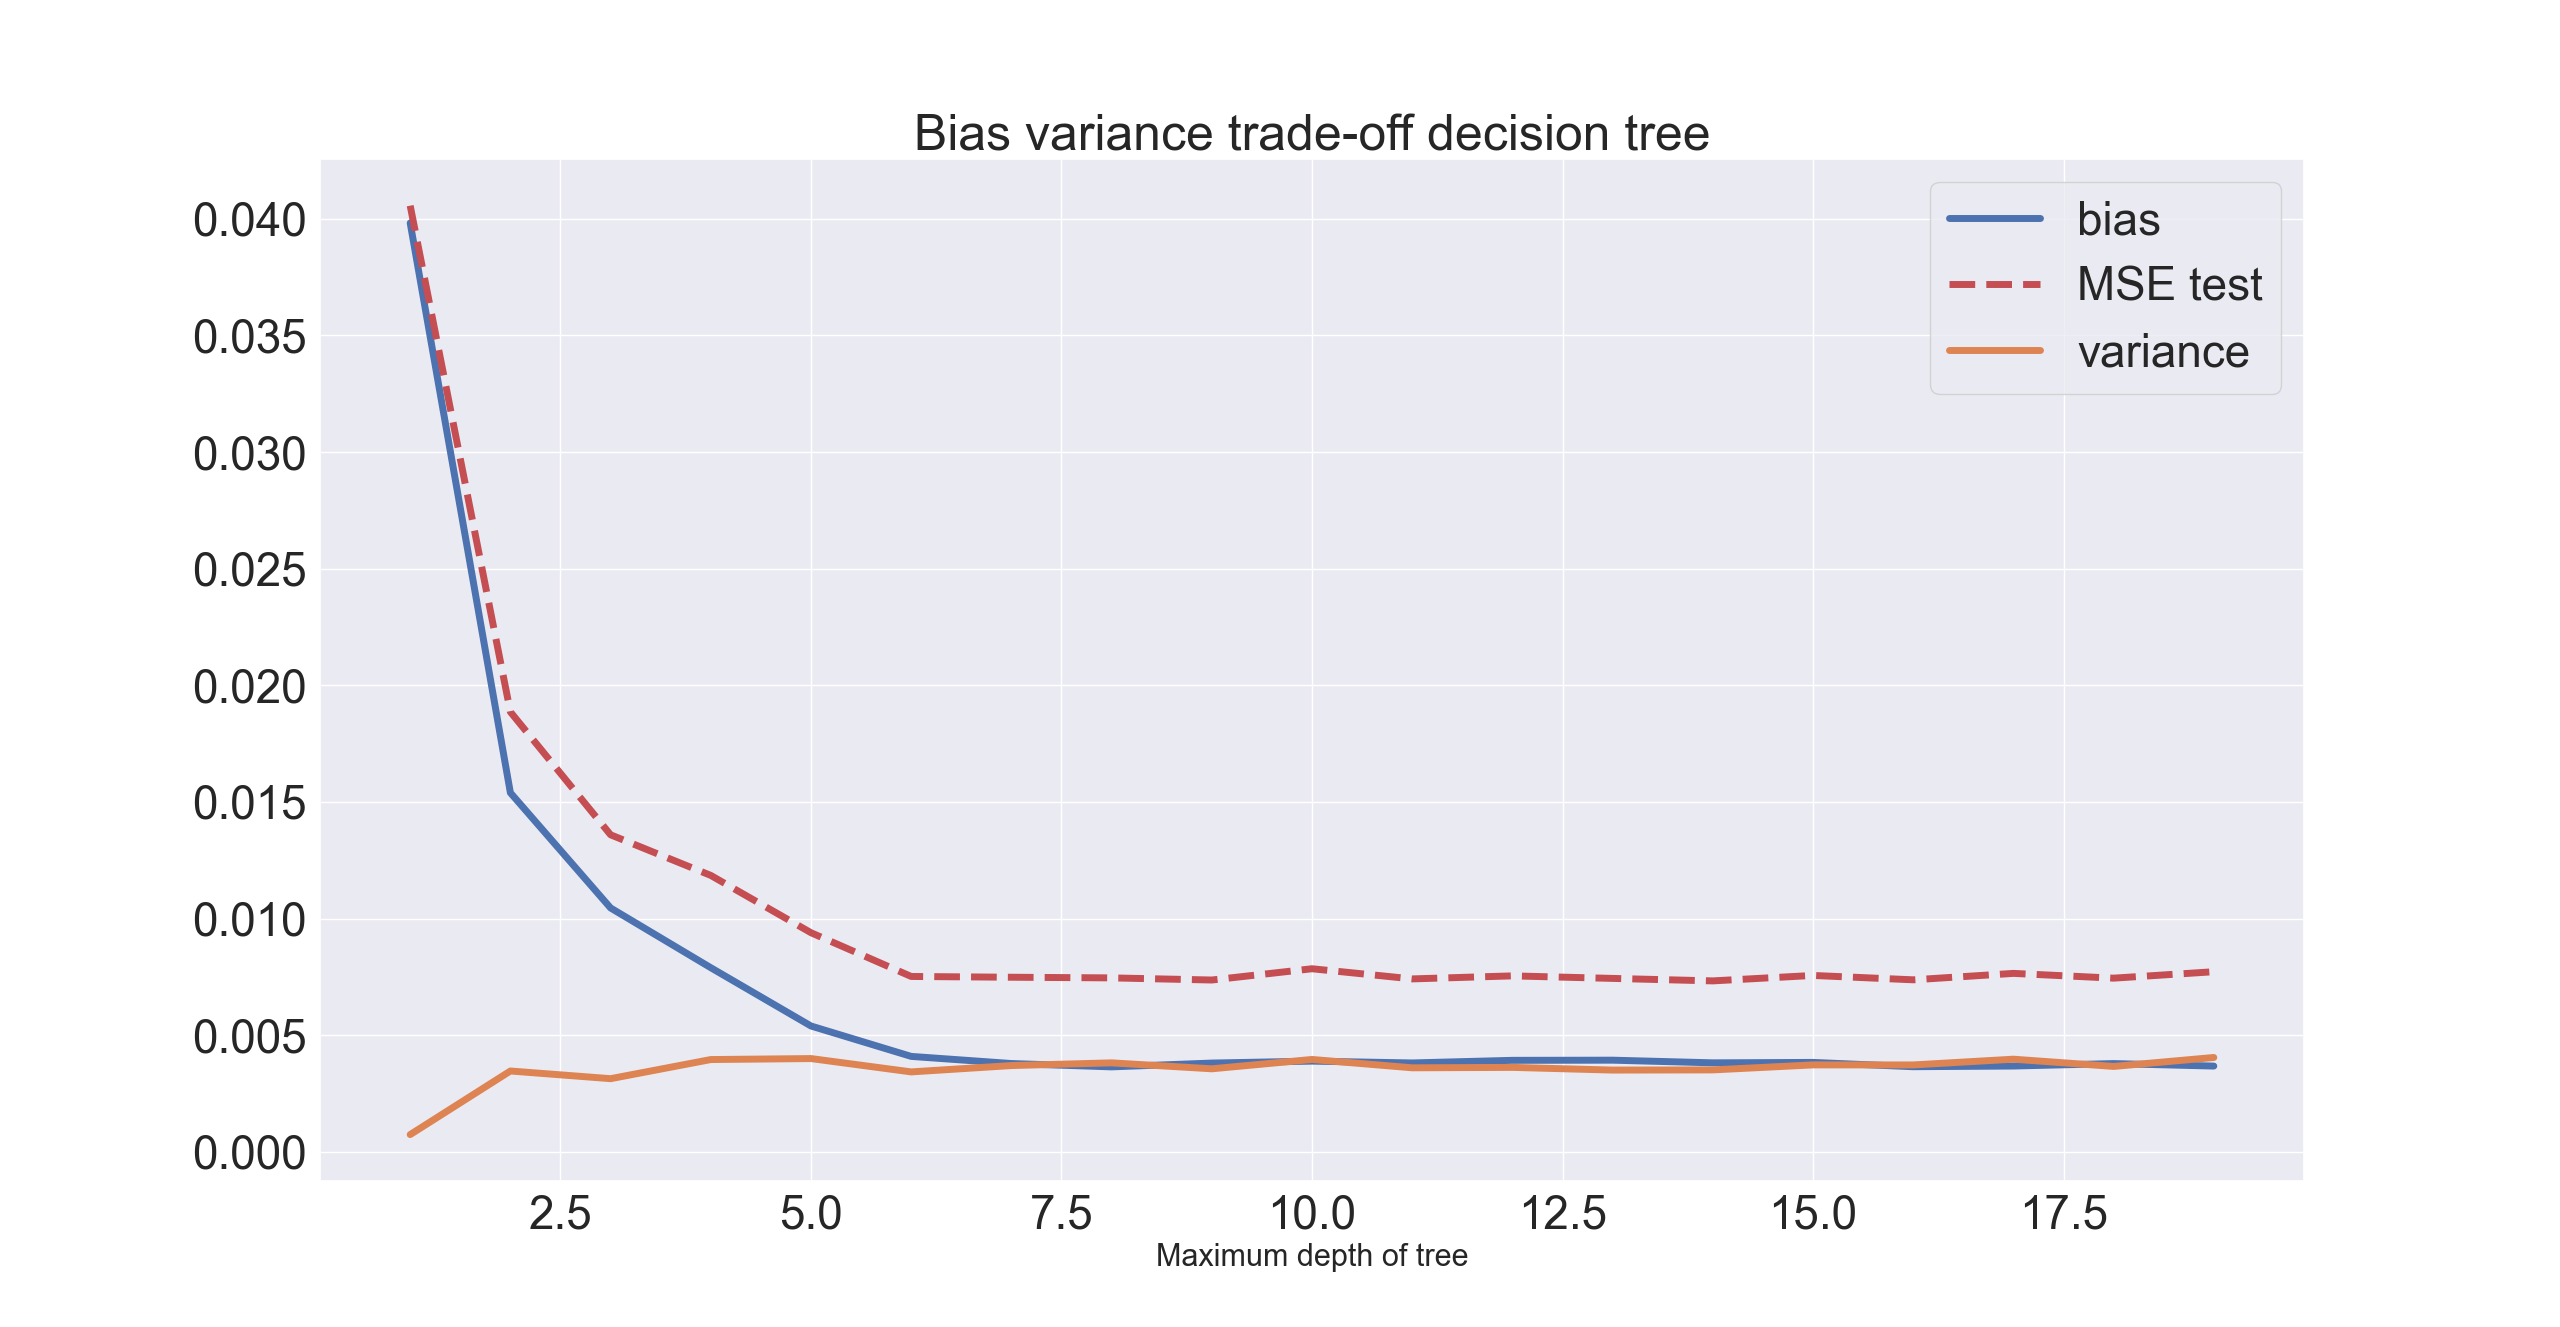
\includegraphics[width=5in]{figs/BV_Decison_tree.png}}
\caption{Bias variance trade-off for decision tree regressor. Y axis represents model complexity as max depth.}
\label{tree}
\end{figure}

Looking at a completely different way of performing our regression, the decision tree model provides interesting results. Looking at (Fig.~\ref{tree}), the bias variance trade-off is much different, as the variance increases much more and the bias decreases less. This yields a higher bias and variance, and since the MSE can be expressed as the sum of both these factors, this provides a larger test mean squared error. The decision tree regressor yields an MSE of 0.0077, over double that of our best result using ridge regression. Though it does not appear to overfit our training data, the decision tree does not provide impressive results for our regression case. The fact that decision trees are very explainable does not provide a useful argument for selecting the decision tree model, as we are dealing with conditions based on numbers which yield little intuition.

\begin{figure}[H]
\centerline{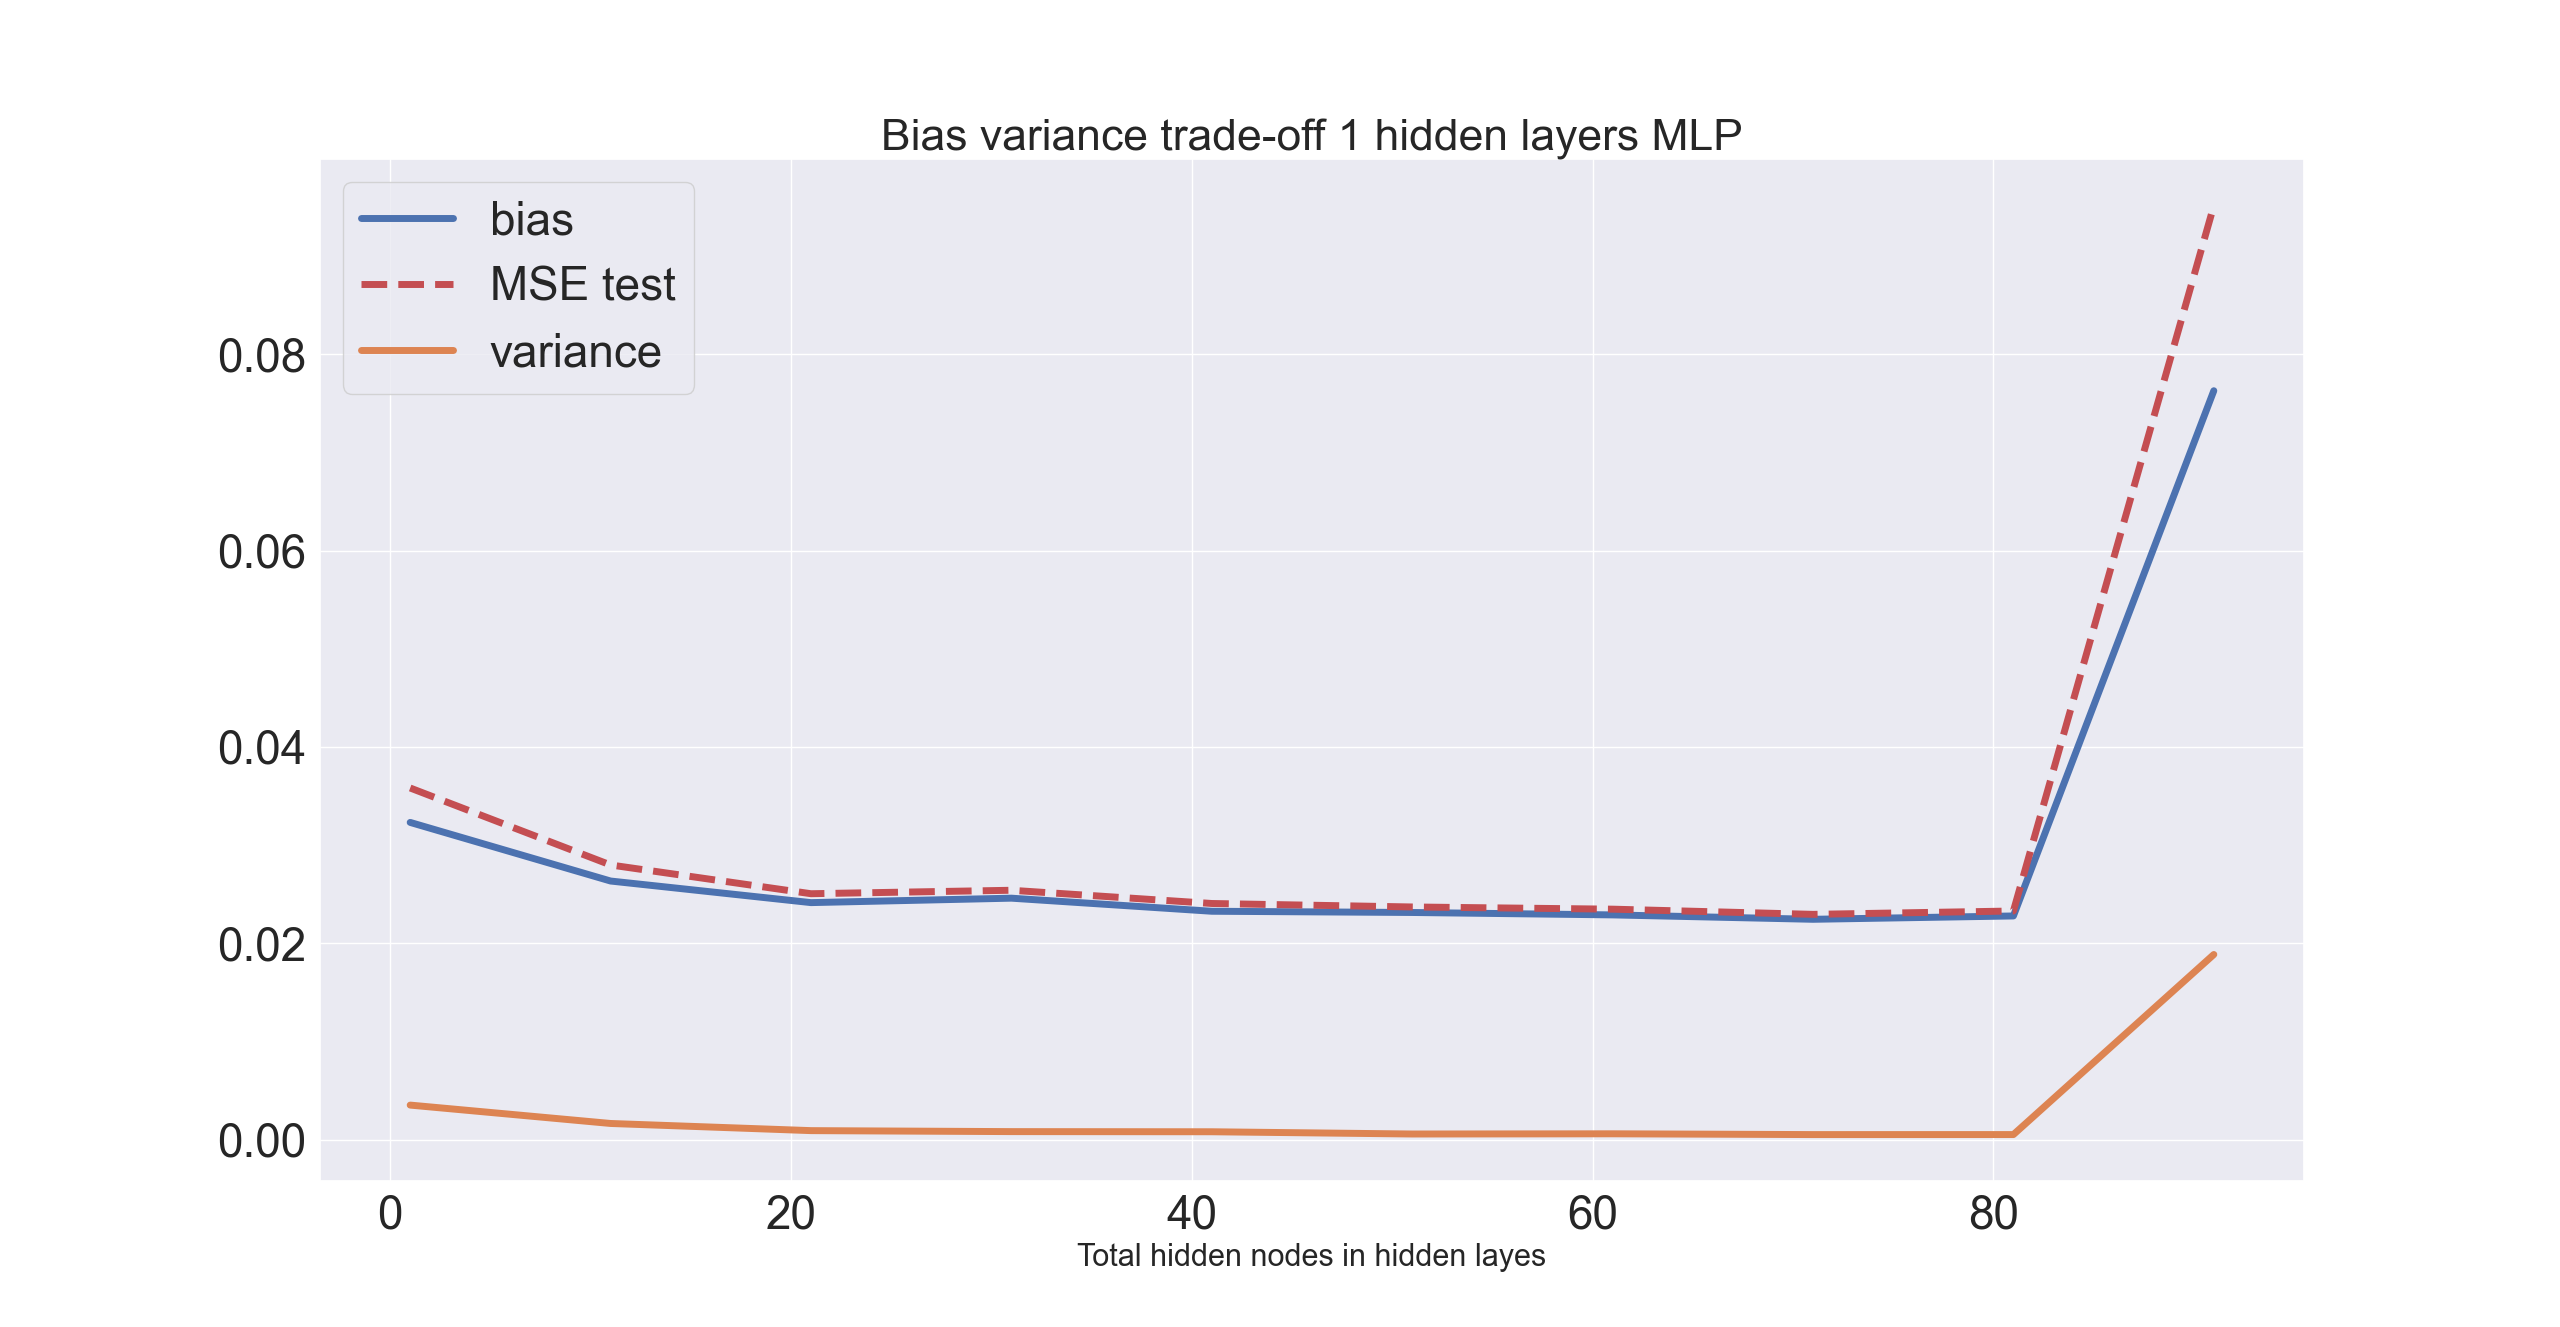
\includegraphics[width=5in]{figs/BV_ffnn1.png}}
\caption{Bias variance trade-off for feed forward neural network with one hidden layer. Y axis represents model complexity as nodes present in the hidden layers.}
\label{ffnn1}
\end{figure}

For the feed forward neural network, we can see from (Fig.~\ref{ffnn1}) that a FFNN with one hidden layer will overfit when the hidden layer contains over 80 hidden nodes. The test MSE reaches a minimum of 0.022, a whole order of magnitude worse than our previous results. Unsatisfied with this result, we turn to an architecture with more hidden layers in a persuit of a lower MSE. Strangely, the cause of the MSE increasing for hidden node counts greater than 80 is a large increase in the bias. Typically, the bias will start high and go downwards as the model complexity increases. This might be because the FFNN simplifies the relationship learned to describe the pattern, increasing the bias. The variance does also increase however, but not as much as the bias.

\begin{figure}[H]
\centerline{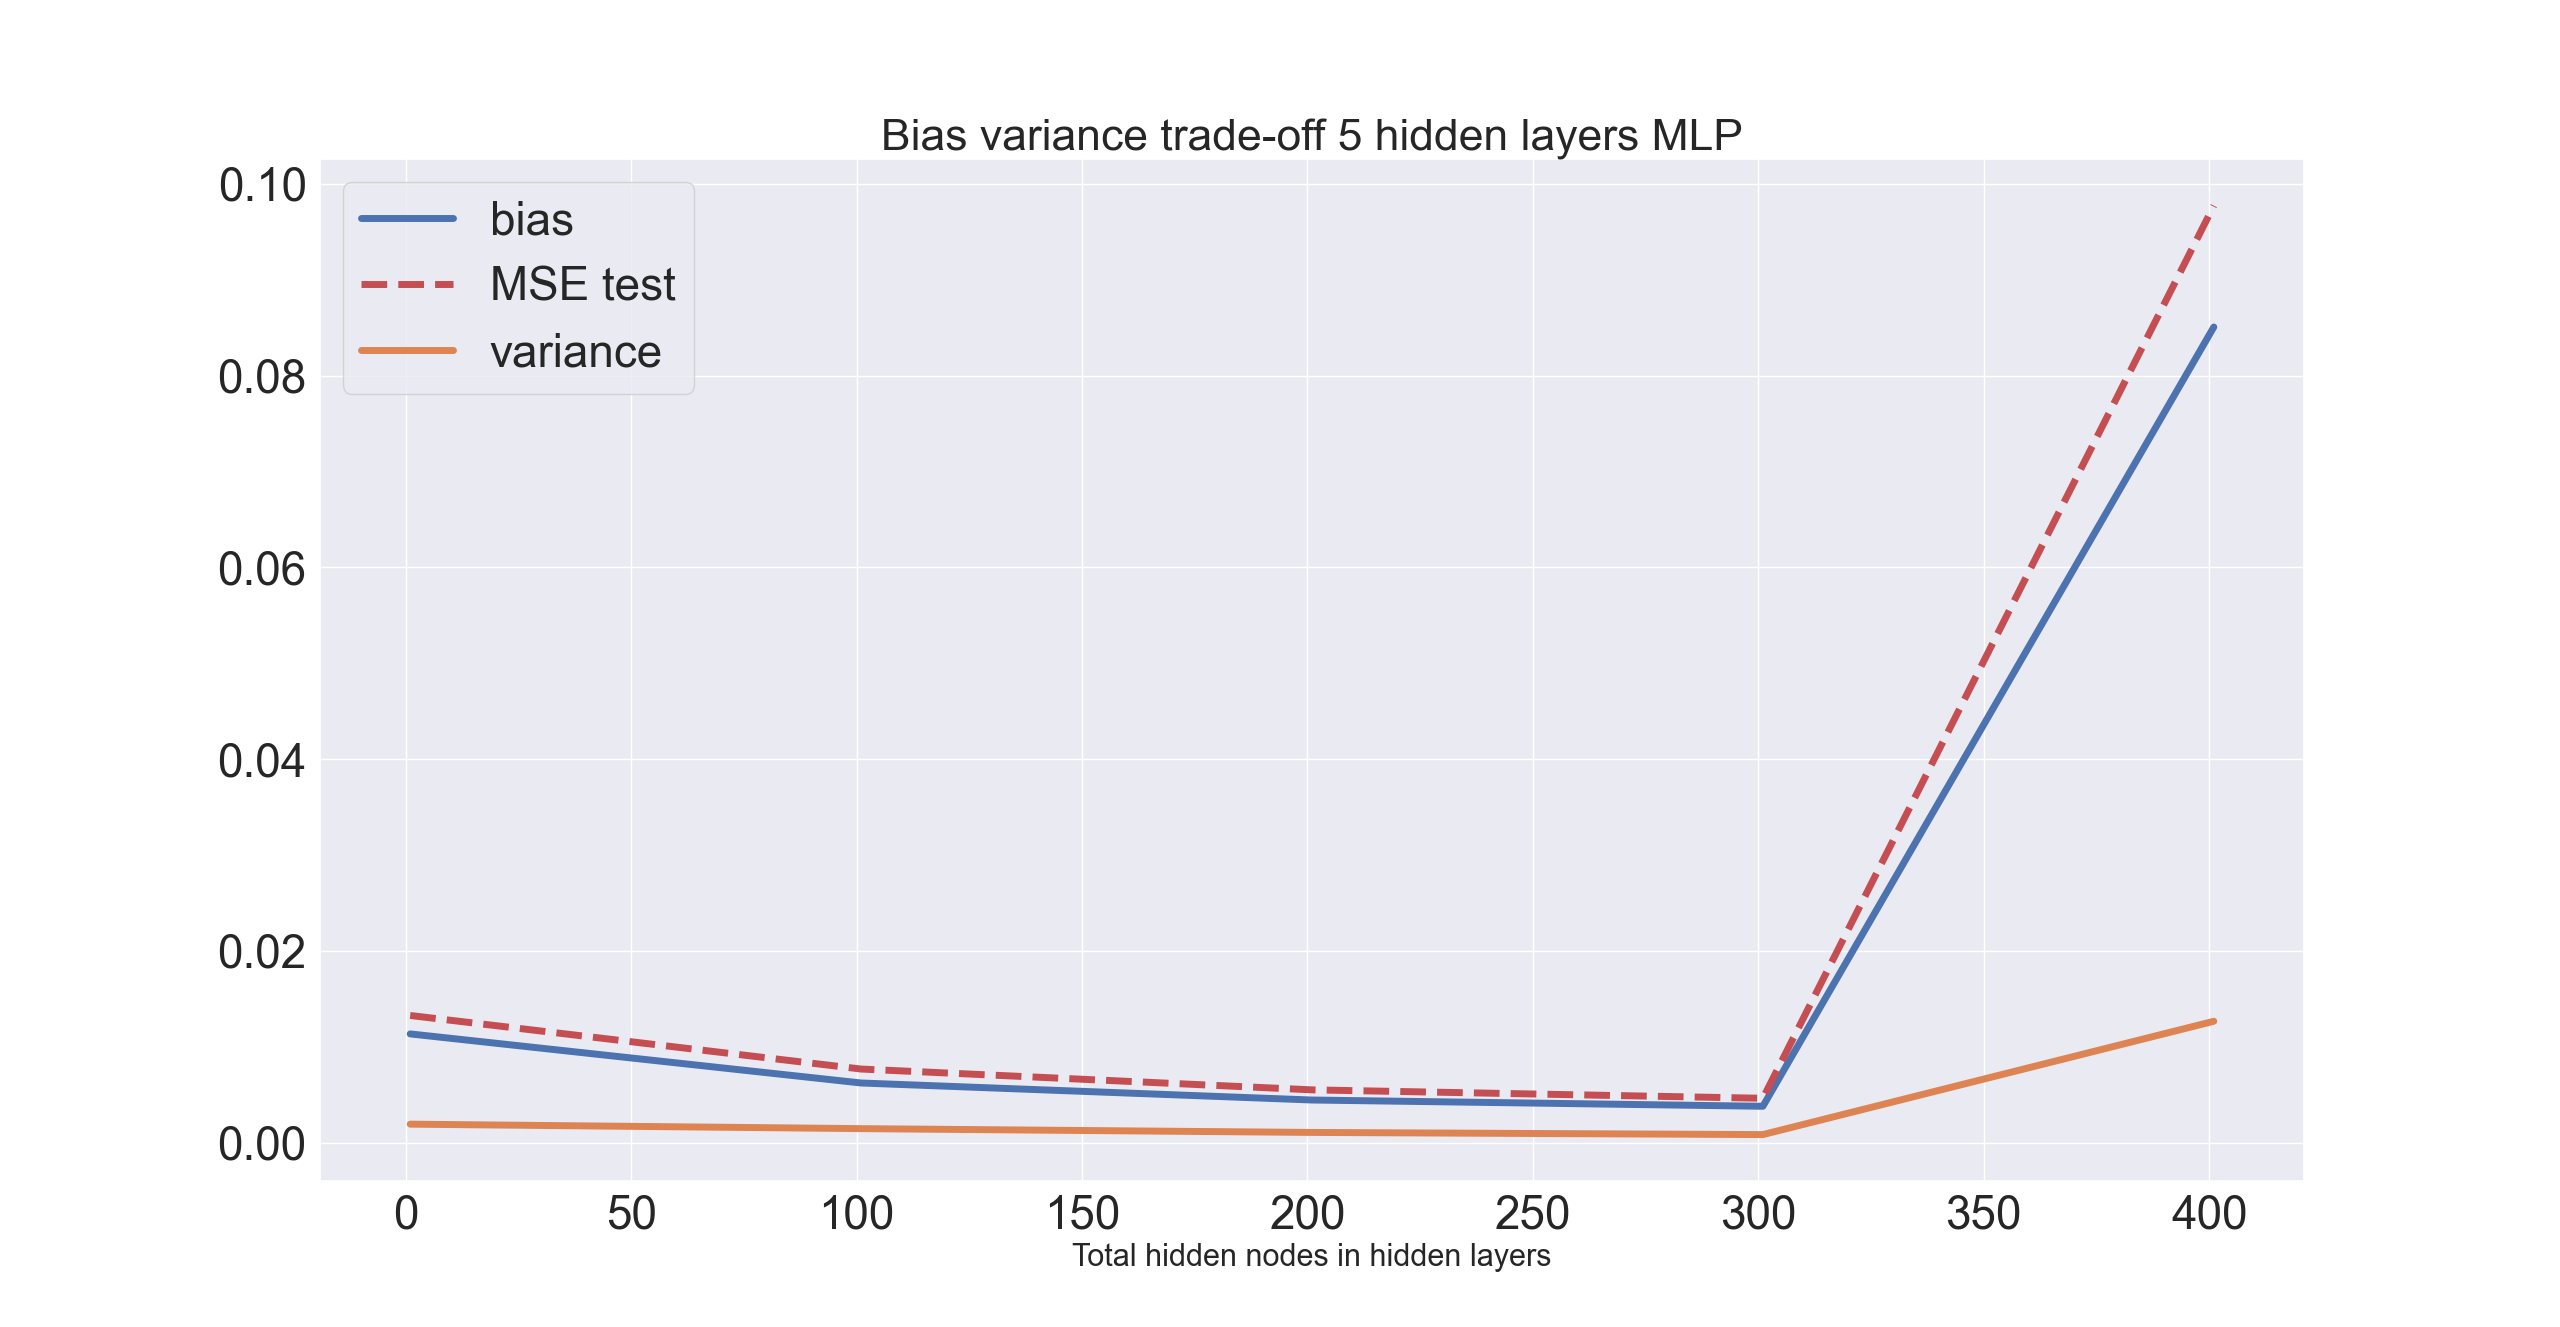
\includegraphics[width=5in]{figs/BV_ffnn5.png}}
\caption{Bias variance trade-off for feed forward neural network with 5 hidden layers. Y axis represents model complexity as nodes evenly distributed in the hidden layers.}
\label{ffnn5}
\end{figure}

By increasing the amount of hidden layers to 5 hidden layers, we are able to achieve a much better test MSE of 0.0050 with 60 hidden nodes per hidden layer as seen in (Fig.~\ref{ffnn5}). However, allthough we have decreased the MSE with a whole order of magnitude when compared to a neural network with one hidden layer, the model complexity and computational cost has also greatly increased. When compared to OLS and ridge, the computational cost of the 5 layer FFNN is much greater whilst the MSE is 61\% higher than the MSE obtained from ridge regression. This is a poor result. Again, the MSE increases mainly because of an increase in bias along with an additional increase in variance. Graphs of the bias variance trade-off for 3 and 7 hidden layers, which don't improve upon the result.

\subsection{Conclusion}
Ridge proved to be the best regression model, as the regularization allows us to drive down the MSE to an impressive 0.0031 whilst delaying the overfitting. Ridge was able to mentain a low bias and variance, an impressive 14\% decrease from OLS' results. Decision trees didn't overfit, but was unable to beat the MSE of ridge and OLS as the bias variance trade-off featured both a higher bias and variance. The FFNN required a great increase in computational cost whilst not being able to beat the MSE of OLS and Ridge. For 5 hidden layers, the FFNN yields a lower MSE than the decision tree.

Further research on this topic could include more varying architectures of the feed forward neural network, along with different regression models like support vector machines.

\bibliographystyle{apalike}
\bibliography{bibliography}

\section*{Appendix A: Plots and reproducibility}

The next page contains information on how to reproduce the plots in this paper along with additional figures.

\begin{table*}[h]
\caption{This table shows the file which created every plot in the report}
\begin{center}
\label{allparamstable}
\begin{tabular}{c | l l l}
Figure & Shell command \\
\hline
\ref{OLS} & \texttt{python3 OLS\_bias\_variance.py}\\
\ref{Ridge} & \texttt{python3 ridge\_bias\_variance.py}\\
\ref{tree} & \texttt{python3 decision\_tree\_bias\_variance.py}\\
\ref{ffnn1} & \texttt{python3 ffnn\_bias\_variance.py}\\
\ref{ffnn2} & \texttt{python3 ffnn\_bias\_variance.py}\\
\hline
\end{tabular}
\end{center}
\end{table*}

\begin{figure}[H]
\centerline{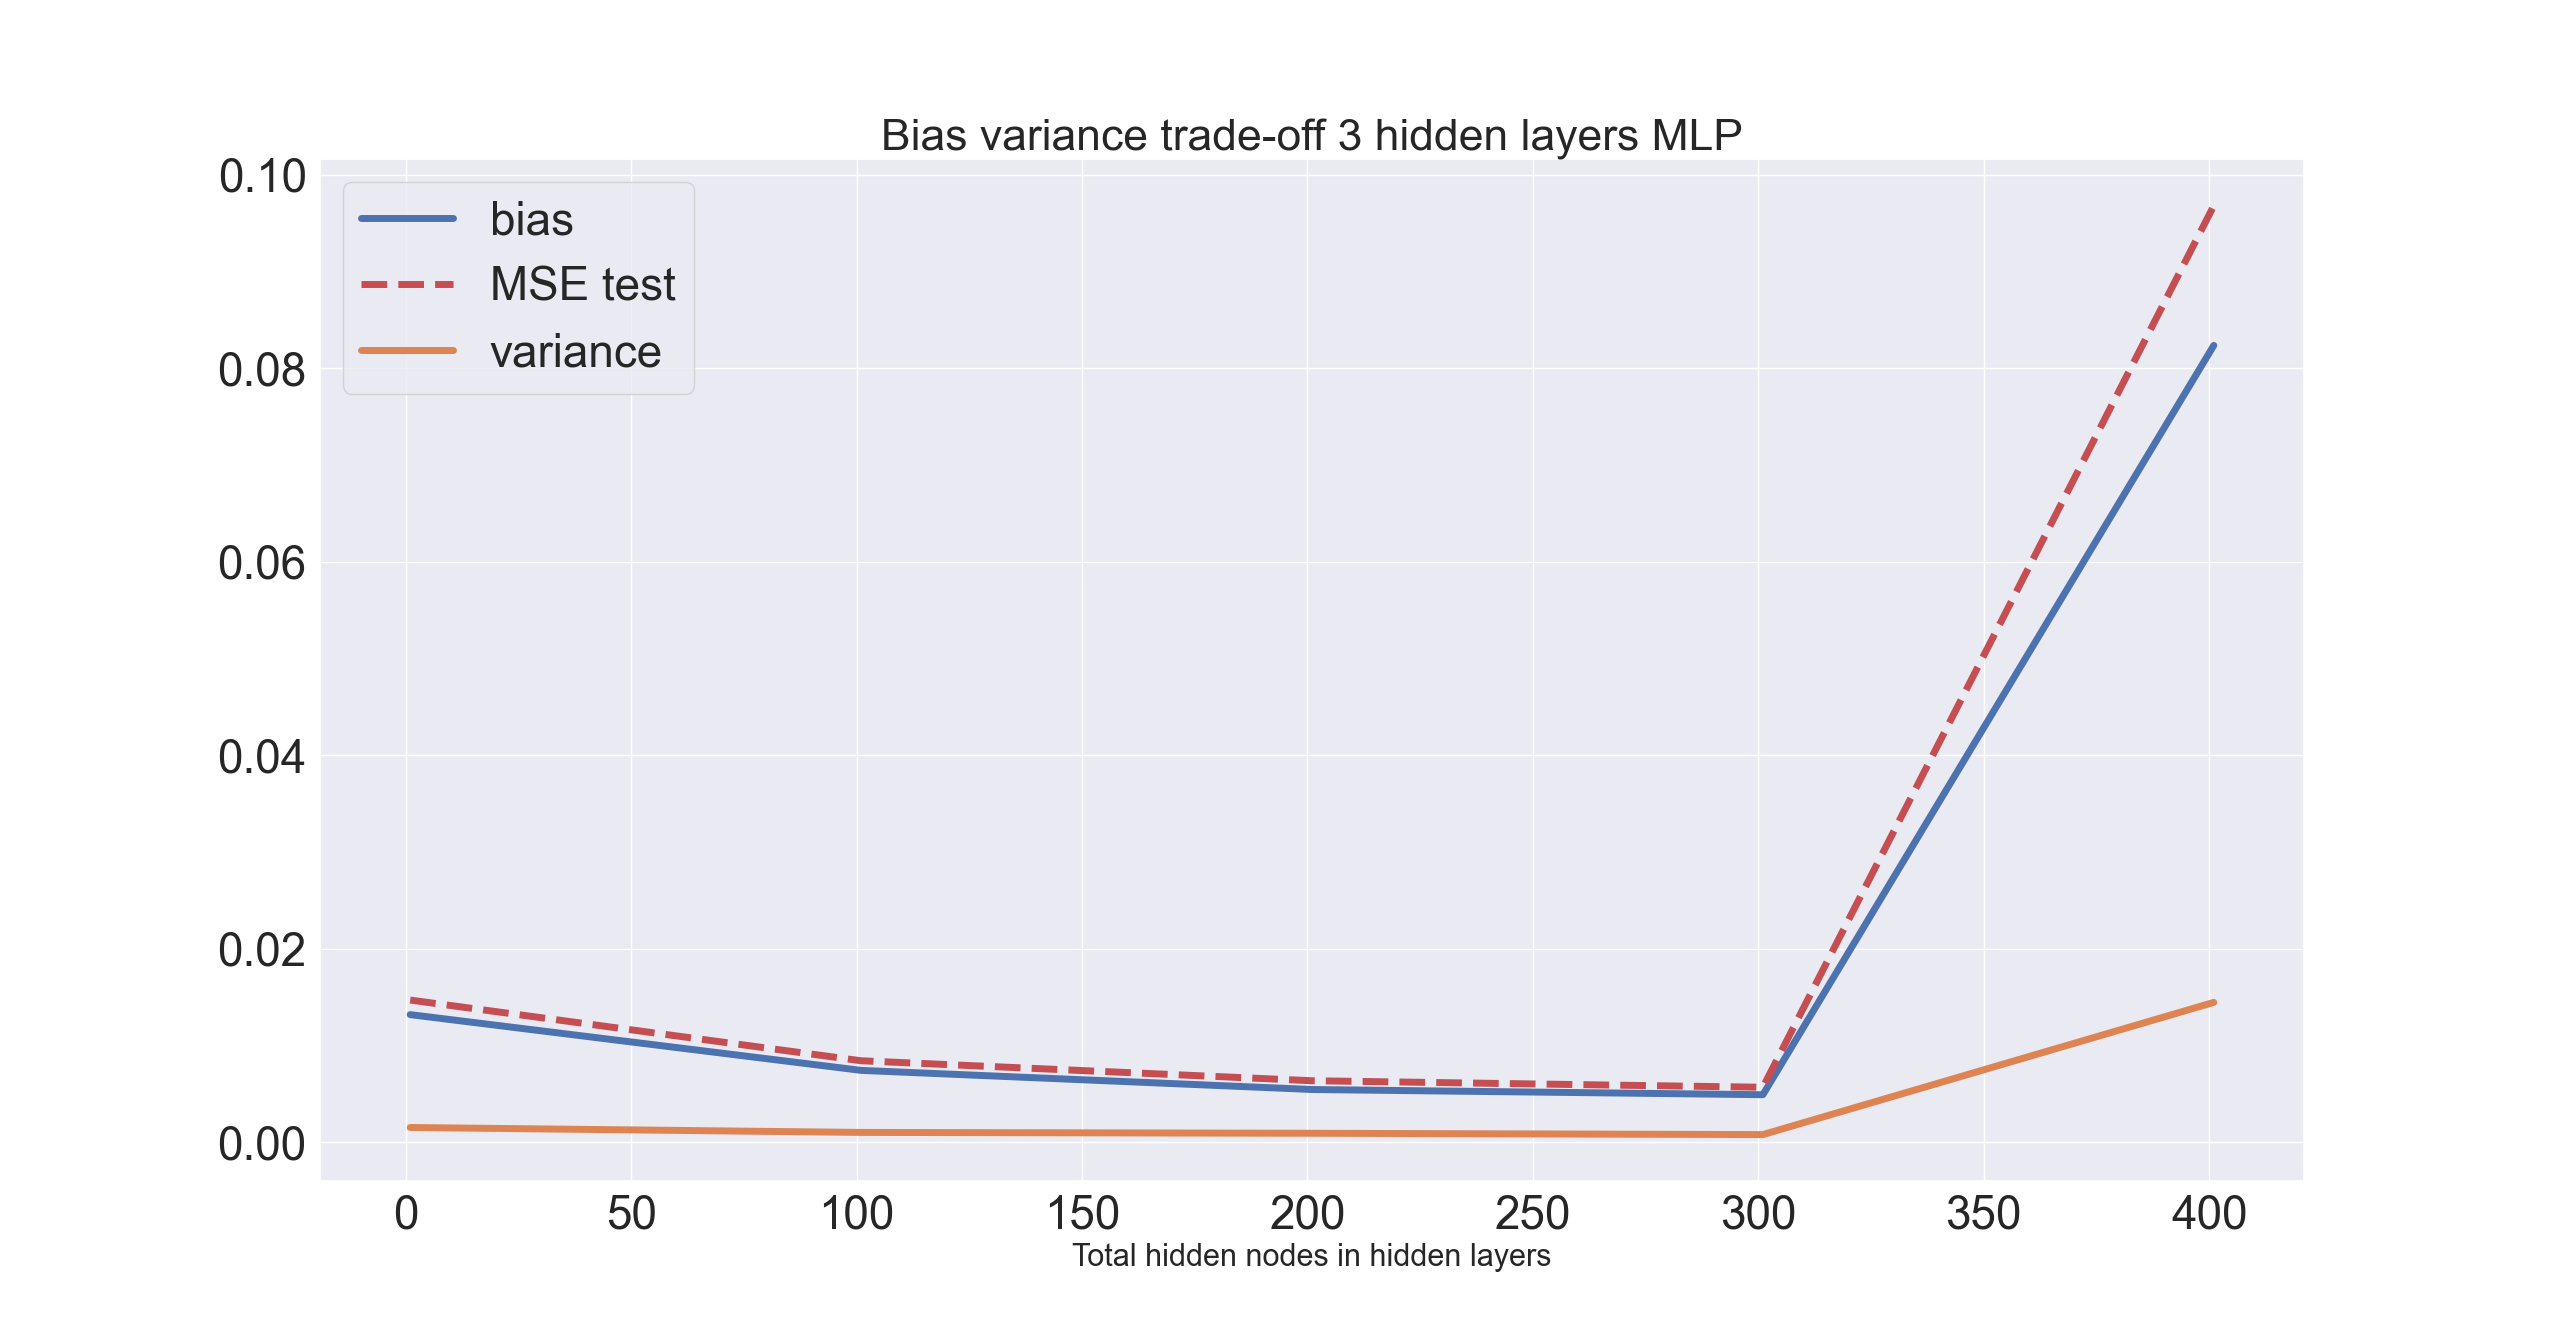
\includegraphics[width=5in]{figs/BV_ffnn3.png}}
\caption{Bias variance trade-off for feed forward neural network with 3 hidden layers. Y axis represents model complexity as nodes evenly distributed in the hidden layers.}
\label{ffnn5}
\end{figure}

\begin{figure}[H]
\centerline{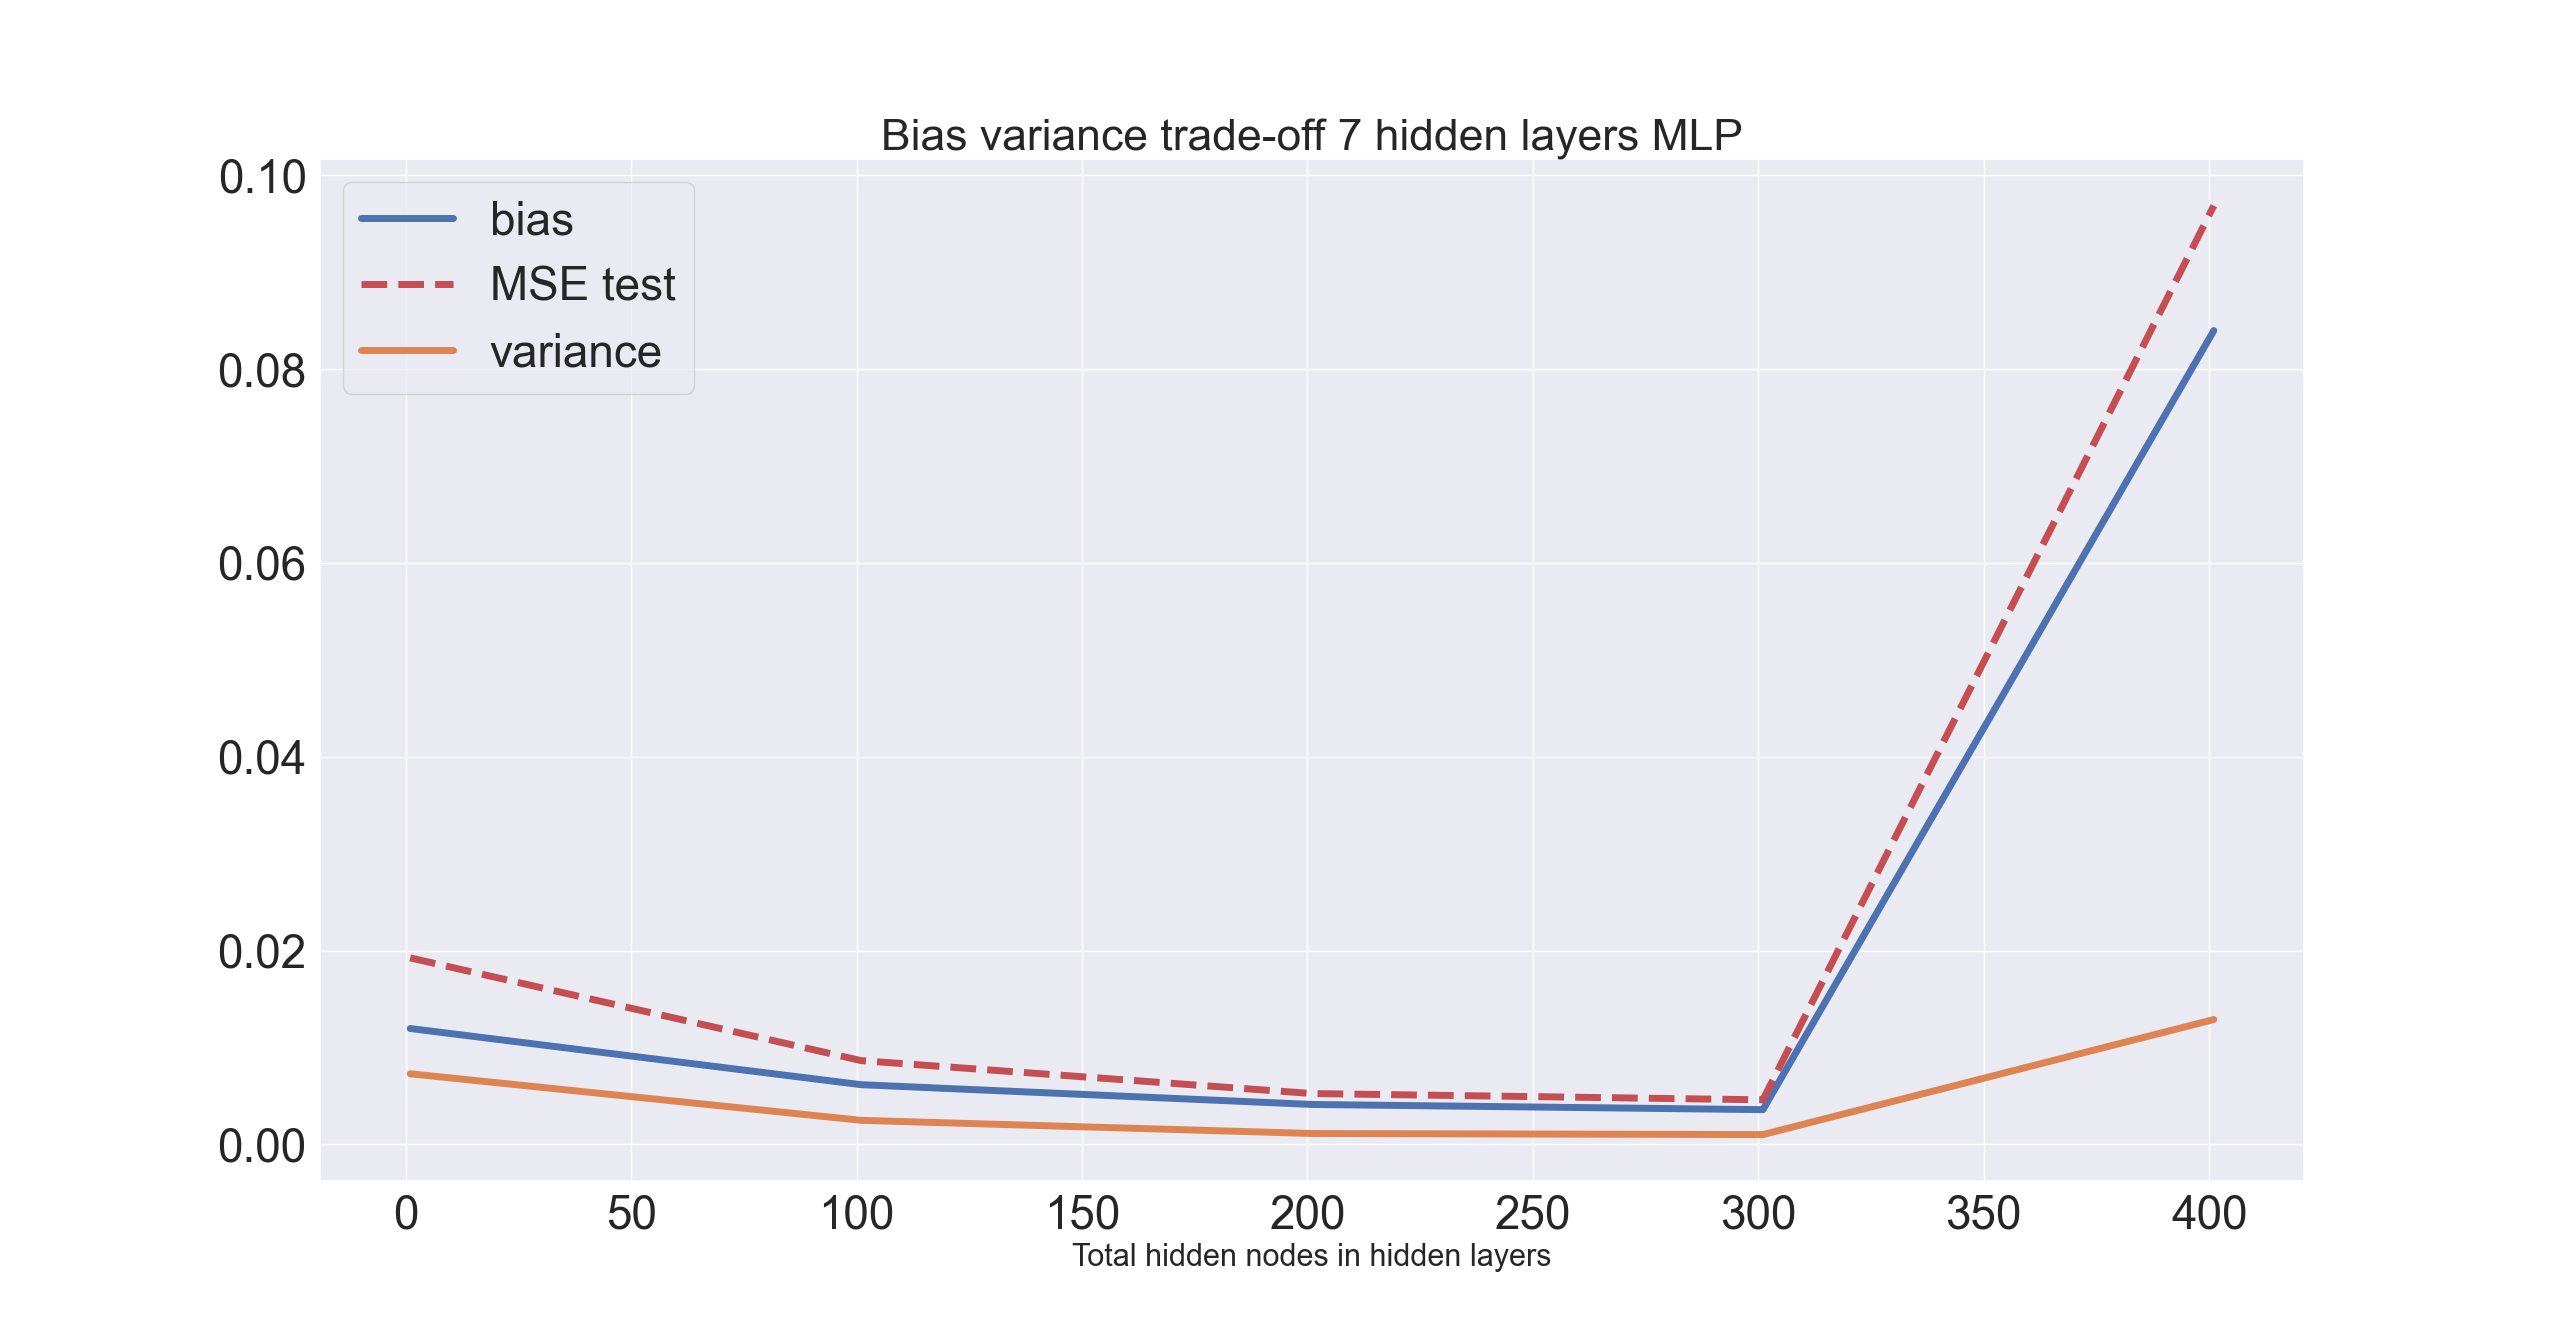
\includegraphics[width=5in]{figs/BV_ffnn7.png}}
\caption{Bias variance trade-off for feed forward neural network with 7 hidden layers. Y axis represents model complexity as nodes evenly distributed in the hidden layers.}
\label{ffnn5}
\end{figure}

\end{document}